\documentclass{tufte-handout}
\usepackage{graphicx}
\usepackage{amsmath}
\graphicspath{ {../images/} }
\renewcommand{\vec}[1]{\mathbf{#1}}

\title{Final Exam Review Notes}
\author{Andr\'es Ponce}

\begin{document}
\maketitle

%modify this plz :'(
\begin{abstract}
	All the topics from classification, regression, and different models for 
	each will be covered.

\end{abstract}
\section{Linear Models for Classification}
In supervised learning, we might have scenarios where we have an input vector $\vec{x}$
Given some of the training data, we would like to assign $\vec{x}$ to possibly $k$ classes.
There are some different approaches:
\begin{enumerate}
	\item \textbf{Discriminant Functions}:
			\footnote{Yikes!}
			Here we have a function whose output value indicates which class the data point gets assigned to.
			For example, if a function has a value greater than $y$, then we assign it to one class, and 
				another class otherwise.
			Basically, it would amount to having an equation like
			\[ \begin{cases}
					0, & y(x) \leq 0 \\
					1 & y(x) > 0 \\
				\end{cases}
			\]
	\item \textbf{Generative approach}
			With a generative approach, we try to model the class-conditional probability
			\[p(C_{k}|\vec{x}) = \frac{p(\vec{x}|C_{k})p(C_{k})}{p(\vec{x})}\]
\end{enumerate}

The weight vector $\vec{w}$ lies on orthogonal to the \textbf{decision boundary}, or the boundary that 
	differentiates between being assigned to $C_{1}$ or $C_{2}$.

For multiclass classifiers, we can have a couple different approaches
\begin{enumerate}
	\item \textbf{One-versus-the-rest}: We build $K-1$ classifiers to handle a binary classification. We
			basically ask the question ``Is this point in class $k\in K$, or is it in not?" This means that
			for all classes we can learn a model that basically predicts whether a point will fall in this 
			class or outside. 

			The problem with this approach lies in that there may be \textbf{ambiguous} regions in the input
			space, typically when multiple classifiers predict a point lying outside of their region and then
			it becomes unclear which class exactly they belong to. When one model says ``this point does not lie
			in $C_{k}$, several other classees may be saying this and lead to conflicting spaces.
			\begin{marginfigure}
				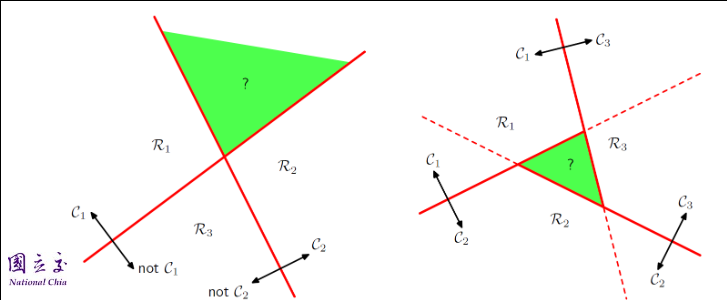
\includegraphics[scale=0.2]{ambiguous}
				\caption{Here, when we map the contents outside of the main class, it can conflict with the
						classification made some of the other models.}
			\end{marginfigure}

	\item \textbf{One-versus-one}
			Here we learn $K(K-1)/2$ models, one for each $(C_{1}, C_{2})$ pair. 
			Thus, we have one model for each combination of pairs, and then the final classification is done
			by majority vote.
			
			How does this avoid ambiguous regions? 

			$j \neq k$.
\end{enumerate}
\subsection{Least Squares for Classification}
	Using  a data point for $\vec{x}$ for classfication, we define $\tilde{x}$ as being $(1, x^{T})^{T}$.
	When we predict a point as belonging to class $k$, we can write it as a 1-0 vector with 1 being the 
	index of the class the point was assigned to, for example $[0,1,0]$ if the point was assigned to 
	the second class out of three.
	
	Least Squares in general are more susceptible to outliers, in that points that lie outside the normal range
	will have more of an effect on the decision boundary, even if the majority of data points lie in a same
	range.

	Another method to do classification is to use \textbf{Fisher's Linear Discriminant}

\subsection{Fisher's Linear Discriminant}
Fisher's Linear Discriminant focuses on the ratio $S$, which is the ratio between the 
\textit{\textbf{between-class variance}} and the \textit{\textbf{between-class variance}}.
		\begin{equation}
		S = \frac{\sigma^{2}_{between}}{\sigma^{2}_{within}}
		\end{equation}

What we want to achieve is a classifier that separates the classes as far as possible.
The weight vector $\vec{w}$ is going to be orthogonal to the decision boundary. 
We are going to project the points onto the decision boundary, and make a decision for our classes based on 
	how the data points actually line up compared to the decision boundary.
The between class variance is defined as 
\[S_{b}\vec{w} = (\vec{m}_{2}-\vec{m}_{1})(\vec{m}_{2}-\vec{m}_{1})^{T}\]

The above vector is in the direction of $\vec{m}_{2}-\vec{m}_{1}$.

Once the data is projected
\footnote{Remeber the projection onto the decision boundary is carried out by $\vec{w}\vec{x}\vec{w}^{T}$}
we can have several ways of actually carrying out the classification. 
We can do a \textbf{threshold}
\footnote{Like in Hw2, we had a value which we used to separate the values in C1 from C2.}
where we just separate the classes based on how they all along that line.

We can also use a \textbf{nearest neighbors rule}, where we predice the class a point belongs to based on 
	the points that are around it, and do a majority vote.

For multiple classes, we have to calculate the mean of all the input vectors, and use that measure for the
	between class variance vector.

\subsection{Perceptron}
The perceptron algorithm functions for two-class classification.
In this algorithm, we first transform the input vector $\vec{x}$ with a function $\phi(x)$. 
We then do
\[ y(x)=f(\vec{w}^{T}\phi(x))\]
where $f(x)$ is the \textbf{activation function}.
This output then maps to $\{-1, 1\}$ depending on which class the point is estimated to belong to.

How do we know if the data point we just classified is correct? 
We can take the product 
\[ \vec{w}^{T}\phi(x_{n})t_{n}\]
and see whether the result is greater than 0. 
Why is this the criterion?
If the result is indeed greater than zero, it means that both the target $\vec{t}$ and the actual classification
	prediction had the same sign value, which means we predicted it correctly (maybe both values are -1, for
	example).

For the perceptron, to get the error we add up all the values that were misclassified, and then add it to the 
	values of the perceptron.

\end{document}
